\documentclass[11pt,a4paper]{article}
\usepackage{color}
\usepackage[usenames,dvipsnames]{xcolor}
\usepackage{tikz}
\usepackage[labelformat=empty]{caption}
\usepackage[normalem]{ulem}
\usepackage{subfigure}
\usetikzlibrary{calc}
\usepackage{pgfplots}
\usepackage{amsfonts}
\usetikzlibrary{shapes}
\usetikzlibrary{arrows}
\usetikzlibrary{positioning}
\usepackage[left=1in, right=1in,top=1in]{geometry}

\definecolor{BreakfastRed} {RGB}{227,53,70}
\definecolor{BreakfastGreen} {RGB}{89,112,21}
\definecolor{BreakfastBlue} {RGB}{41,41,97}

\begin{document}

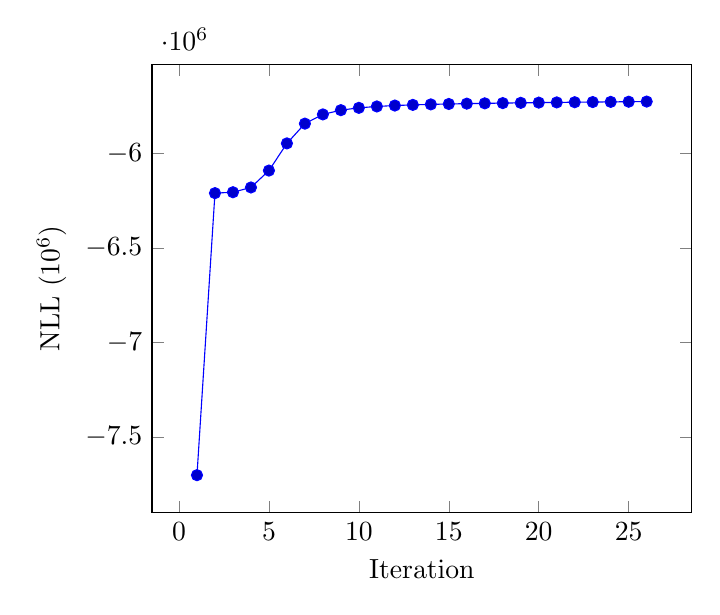
\begin{tikzpicture}
\begin{axis}[
xlabel=Iteration,
ylabel=NLL ($10^6$),
]
\addplot+[sharp plot] coordinates
{(1, -7701462.4701622184) (2, -6210184.4073309442) (3, -6205394.5569028025) (4, -6180189.7077674549) (5, -6090880.6790311793) (6, -5947133.5874003926) (7, -5842658.2770349756) (8, -5793884.1557854749) (9, -5771421.7320397384) (10,  -5759230.7711939001) (11,  -5751889.5108164595) (12,  -5746994.4279526304) (13,  -5743549.4373938348) (14,  -5740916.1159969969) (15,  -5738766.2804557504) (16,  -5736984.2883843854) (17,  -5735397.2103813021) (18,  -5734034.4766451316) (19,  -5732720.4891721541) (20,  -5731546.8076370759) (21,  -5730448.0771911489) (22,  -5729455.4693525182) (23,  -5728518.9275988322) (24,  -5727645.4971987745) (25,  -5726786.2998804012) (26,  -5725959.6553079840)};
\end{axis}
\end{tikzpicture}

\end{document}